\documentclass[a4paper, 12pt, oneside]{book}
\usepackage[italian]{babel} % Lingua italiana
\usepackage{authblk} % Per gli autori

\renewcommand\Authands{ e }

\title{Analisi empirica degli algoritmi di ordinamento}

\author[ ]{Graziano Francesco \thanks{Email: graziano.francesco@spes.uniud.it, Matricola: 166680}}
\author[ ]{Ongaro Michele \thanks{Email: ongaro.michele@spes.uniud.it, Matricola: 168049}}
\author[ ]{Petri Riccardo \thanks{Email: petri.riccardo@spes.uniud.it, Matricola: 167623}}
\author[ ]{Ungaro Marco \thanks{Email: ungaro.marco@spes.uniud.it, Matricola: 168934}}

\affil[ ]{Università degli Studi di Udine, Dipartimento di Matematica e Informatica}

\date{A.A. 2024-2025}
%\date{}

\usepackage{amsmath} % Per equazioni avanzate
\usepackage{amssymb} % Simboli matematici
\usepackage{graphicx} % Per immagini
\usepackage{lmodern} % Font simile a Computer Modern
\usepackage{geometry} % Per margini personalizzati
\usepackage{listings} % scrivere codice
\usepackage{float} % Per il posizionamento delle immagini

\geometry{a4paper, margin=2.5cm}
\cleardoublepage

\begin{document}

\renewcommand{\contentsname}{Contenuti}
\renewcommand{\chaptername}{Capitolo}

\maketitle % copertina del documento
\tableofcontents % sommario di tutti i titoli

\chapter{Introduzione}\label{chap:Introduzione} % (fold)

Il progetto richiede l'implementazione di quattro algoritmi di ordinamento per array interi di dimensioni variabili.
Gli algoritmi che andremo ad analizzare sono il Counting Sort, il Quick Sort, il Quick Sort 3 way e il Radix Sort (algoritmo a scelta).
Oltre alla corretta implementazione viene richiesto di effettuare un analisi empirica dei tempi medi di esecuzione degli algorimti al variare della dimensione dell'array e del range dei valori interi.
Per stimare i tempi di esecuzione di questi algoritmi garanantendo un errore relativo massimo pari a 0.001 adotteremo le seguenti metodologie:
\begin{itemize}
    \item Utilizzeremo un clock di sistema monotono per garantire precisione nelle misurazioni (ad esempio, \texttt{perf\_counter()} del modulo \(time\) in Python);
    \item Andremo a generare almeno 100 campioni per ciascun grafico, con i valori dei parametri (dimensione dell’array \(n\) e intervallo dei valori \(m\)) distribuiti secondo una progressione geometrica;
    \item Effettueremo più esecuzioni per ogni campione, per stimare in modo affidabile il tempo medio di esecuzione e, eventualmente, il relativo errore.
\end{itemize}
Dopo aver stimato i tempi di esecuzione per ciascun algoritmo, risulterà interessante confrontare i grafici ottenuti per analizzare il comportamento degli algoritmi in diverse situazioni, come il caso peggiore, quello migliore o in quello medio.

Da tutto questo potremmo ottenere una verifica empirica dell'andamento asintotico dei tempi di esecuzione di ogni algoritmo.

% chapter Introduzione (end)

\chapter{Counting Sort}\label{chap:Counting Sort} % (fold)

Il Counting Sort è un algoritmo di ordinamento non comparativo: anziché effettuare confronti tra gli elementi, si basa sul conteggio delle occorrenze di ciascun elemento presente nell'array da ordinare.
È particolarmente efficiente quando gli elementi da ordinare sono numeri interi compresi in un intervallo limitato (intervallo \([0, k]\)).
L'implementazione adottata si articola in tre fasi principali:

\begin{itemize}
    \item Conteggio delle occorrenze di ciascun elemento; si costruisce un array ausiliario \(C\) di lunghezza \(k+1\), inizializzato a zero, in cui per ogni elemento \(x\) in \(A\), si incrementa \(C[x]\) di 1.
    \item Calcolo delle posizioni cumulative; per ottenere la posizione finale di ciascun elemento nell'array ordinato, si trasforma \(C\) in un array cumulativo. In questa versione, \(C[0]\) viene inizialmente decrementando di uno, così che \(c[i]\) rapprsenti l'indice massimo in cui si può inserire l'elemento \(i\) nell'array ordinato.
    \item Costruzione dell'array ordinato; si scorre l'array originale da destra a sinistra, e si inserisce ciascun elemento \(x\) nella posizione \(C[x]\) dell'array ordinato, decrementando \(C[x]\) di 1 dopo ogni inserimento. Questo garantisce la stabilità dell'ordinamento, poiché gli elementi con lo stesso valore vengono inseriti nell'ordine in cui appaiono nell'array originale.
\end{itemize}

\noindent Le due funzioni fornite nel codice sono:

\begin{itemize}
    \item \texttt{countingSort(A, B, k)}: scrive l'output ordinato in B;
    \item \texttt{uniformedCountingSort(A, k)}: funzione wrapper che restituisce direttamente una copia ordinata di A.
\end{itemize}

\section{Analisi della complessità}

Siano \(n\) la dimensione dell'array \(A\) e \(k\) il valore massimo contenuto in \(A\). \\

\noindent \textbf{Tempo:}

\begin{itemize}
    \item Conteggio: \(O(n)\) per scorrere l'array \(A\) e contare le occorrenze di ciascun elemento.
    \item Calcolo delle posizioni cumulative: \(O(k)\) per trasformare l'array \(C\) in un array cumulativo.
    \item Costruzione dell'array ordinato: \(O(n)\) per scorrere l'array \(A\) e inserire gli elementi nell'array ordinato \(B\).
    \item Totale: \(O(n + k)\).
\end{itemize}

\noindent \textbf{Spazio:}

\begin{itemize}
    \item Array ausiliario \(C\): richiede \(O(k)\) spazio.
    \item Array ordinato \(B\): richiede \(O(n)\) spazio.
    \item Totale: \(O(n + k)\).
\end{itemize}

\noindent L'algoritmo è efficiente quando \(k = O(n)\), ovvero quando il range massimo dei valori interi è proporzionale alla dimensione dell'array.
In scenari in cui \(k >> n\), il costo della fase di conteggio e l'allocazione dell'array ausiliario \(C\) possono rendere l'algoritmo meno competitivo rispetto ad altri metodi di ordinamento.

\section{Analisi sperimentale}

Sono stati condotti due esperimenti distinti per analizzare le prestazioni empiriche del Counting Sort:

\begin{itemize}
    \item Nel primo esperimento, la dimensione dell'array \(n\) varia, mentre il valore massimo \(k\) è mantenuto fisso a 100000.
    \item Nel secondo esperimento, \(n\) è fissato a 10000, e viene fatto variare \(m\).
\end{itemize}

\noindent In entrambi i casi, i parametri sono stati scelti seguendo una progressione geometrica.
Per ogni valore di \(n\) o \(m\) sono stati generati almeno 100 campioni casuali, ciascuno eseguito più volte per stimare in modo affidabile il tempo medio di esecuzione, mantenendo un errore relativo massimo \(\leq\) 0.001.
Le misurazioni sono state effettuate utilizzando un clock monotono ad alta precisione (\texttt{time.perf\_counter()} in Python).

I risultati ottenuti sono in linea con le aspettative teoriche:
Nel primo grafico (a \(k\) fisso), il tempo cresce linearmente con \(n\), coerentemente con la complessità \(O(n + m)\).
Nel secondo grafico (a \(n\) fisso), il tempo cresce linearmente con \(m\), evidenziando l'impatto della fase di conteggio e dell'allocazione dell'array \(C\).
I due grafici risultanti mostrano visivamente come il Counting Sort si comporti in relazione ai due parametri chiave \(n\) e \(m\).

\section{Grafico dei tempi di esecuzione}

In primo luogo, è stato analizzato l'andamento temporale al variare della dimensione dell'array \(n\), mantenendo costante l'intervallo dei valori a \(k = 100000\). 
Il grafico seguente mostra in:
\begin{itemize}
    \item \textbf{Ascissa}: dimensione \(n\) dell'array (scala logaritmica, \(10^2 \leq n \leq 10^6\)).
    \item \textbf{Ordinata}: tempo di esecuzione (secondi) per l'ordinamento.
\end{itemize}

\begin{figure}[H]
    \centering
    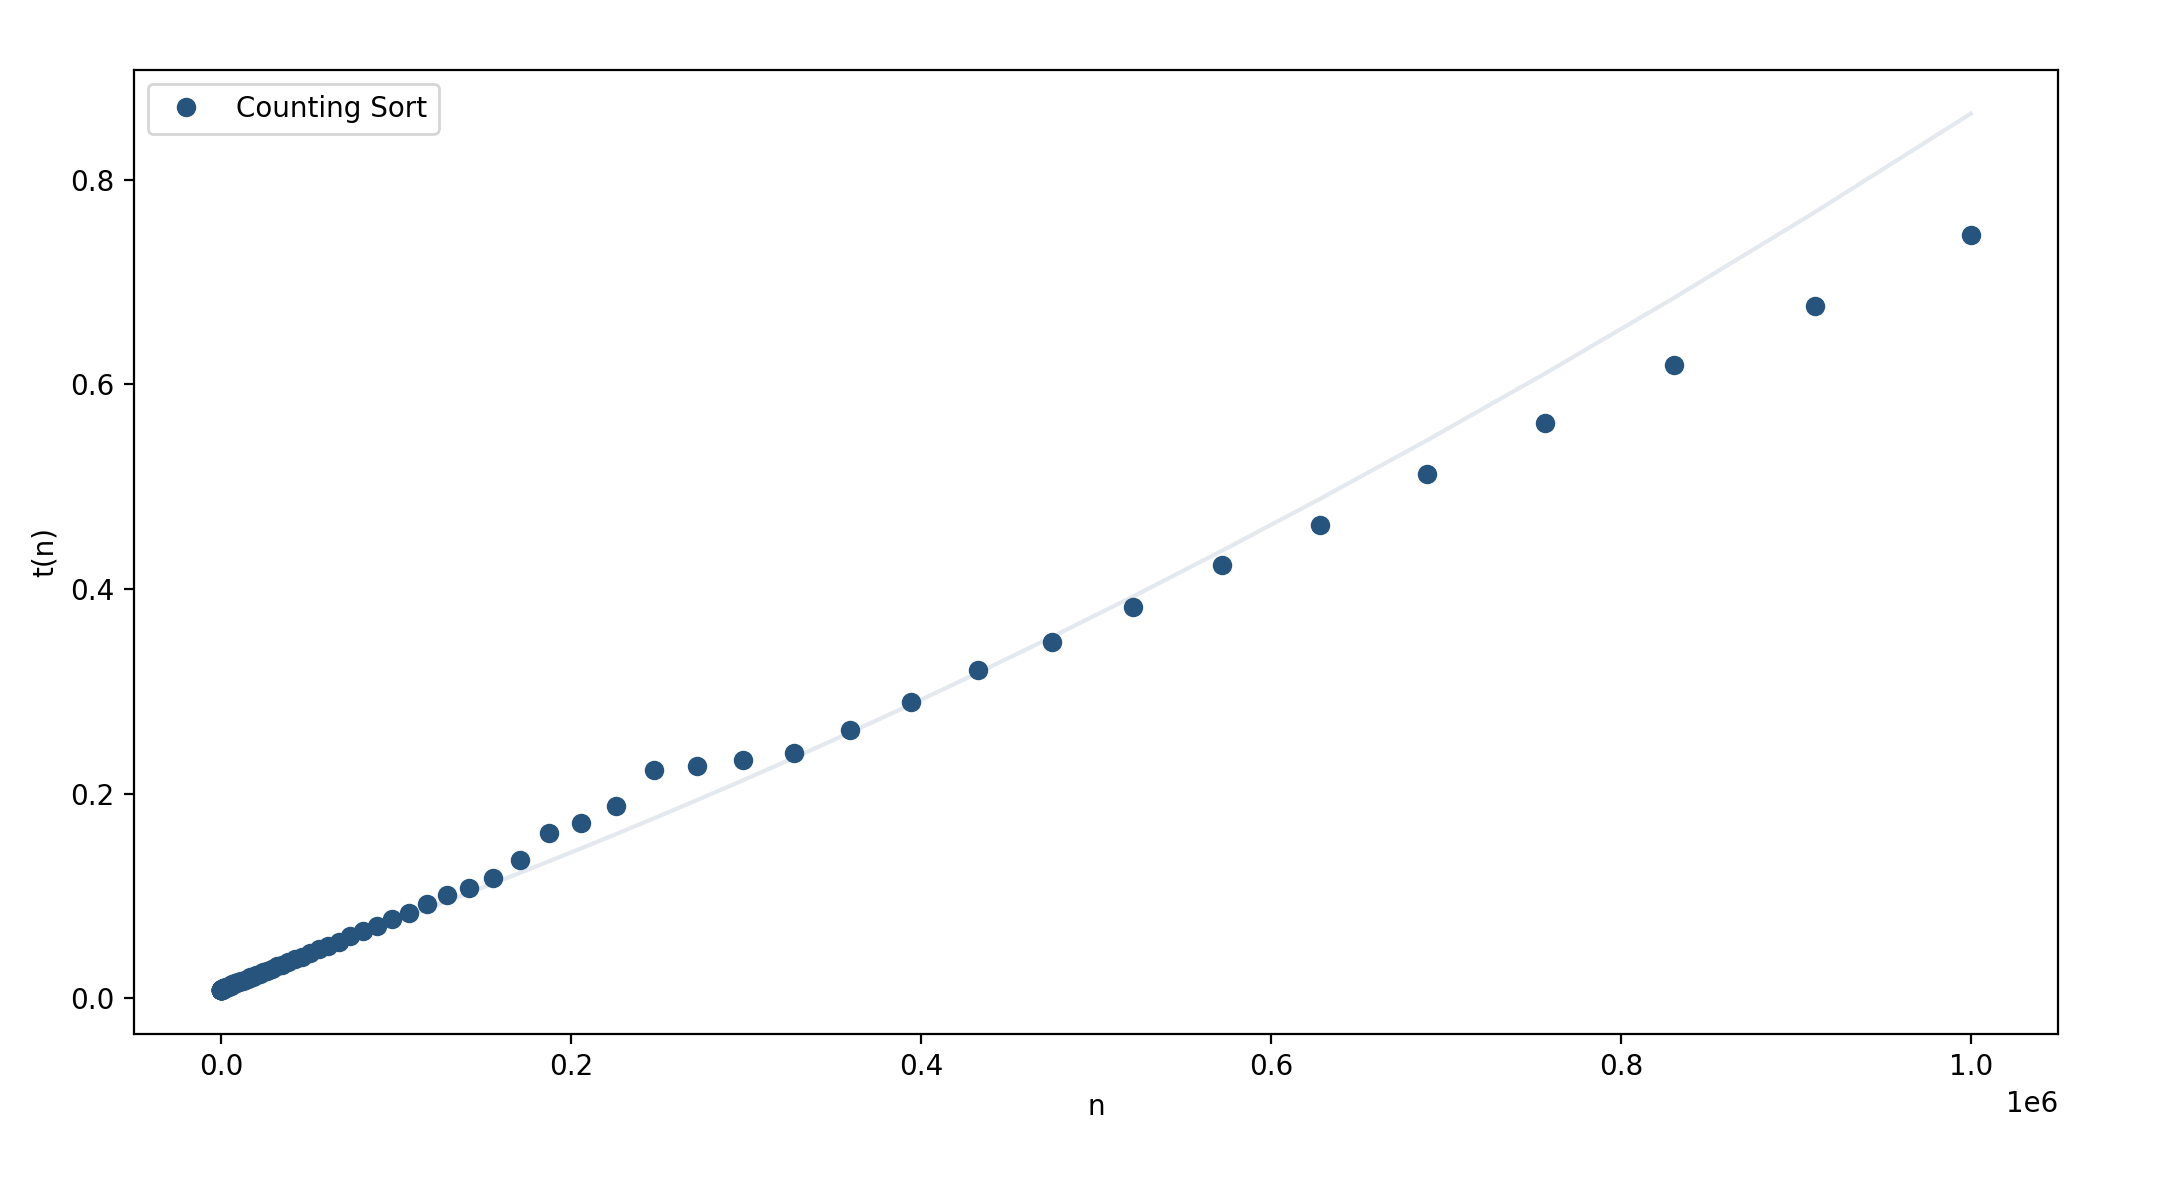
\includegraphics[width=0.8\textwidth]{images/grafico_counting_sort_n.png}
    \caption{Performance del Counting Sort al variare di \(n\).}
    \label{fig:counting_sort_n}
\end{figure}

\noindent Successivamente, è stato analizzato l'andamento temporale al variare dell'intervallo di valori \(m\), mantenendo costante la dimensione dell'array a \(n = 10000\). 
Il grafico seguente presenta:
\begin{itemize}
    \item Ascissa: intervallo \(m\) dei valori (scala logaritmica, \(10^1 \leq m \leq 10^6\))
    \item Ordinata: tempo di esecuzione (secondi) per l'ordinamento
\end{itemize}

\begin{figure}[H]
    \centering
    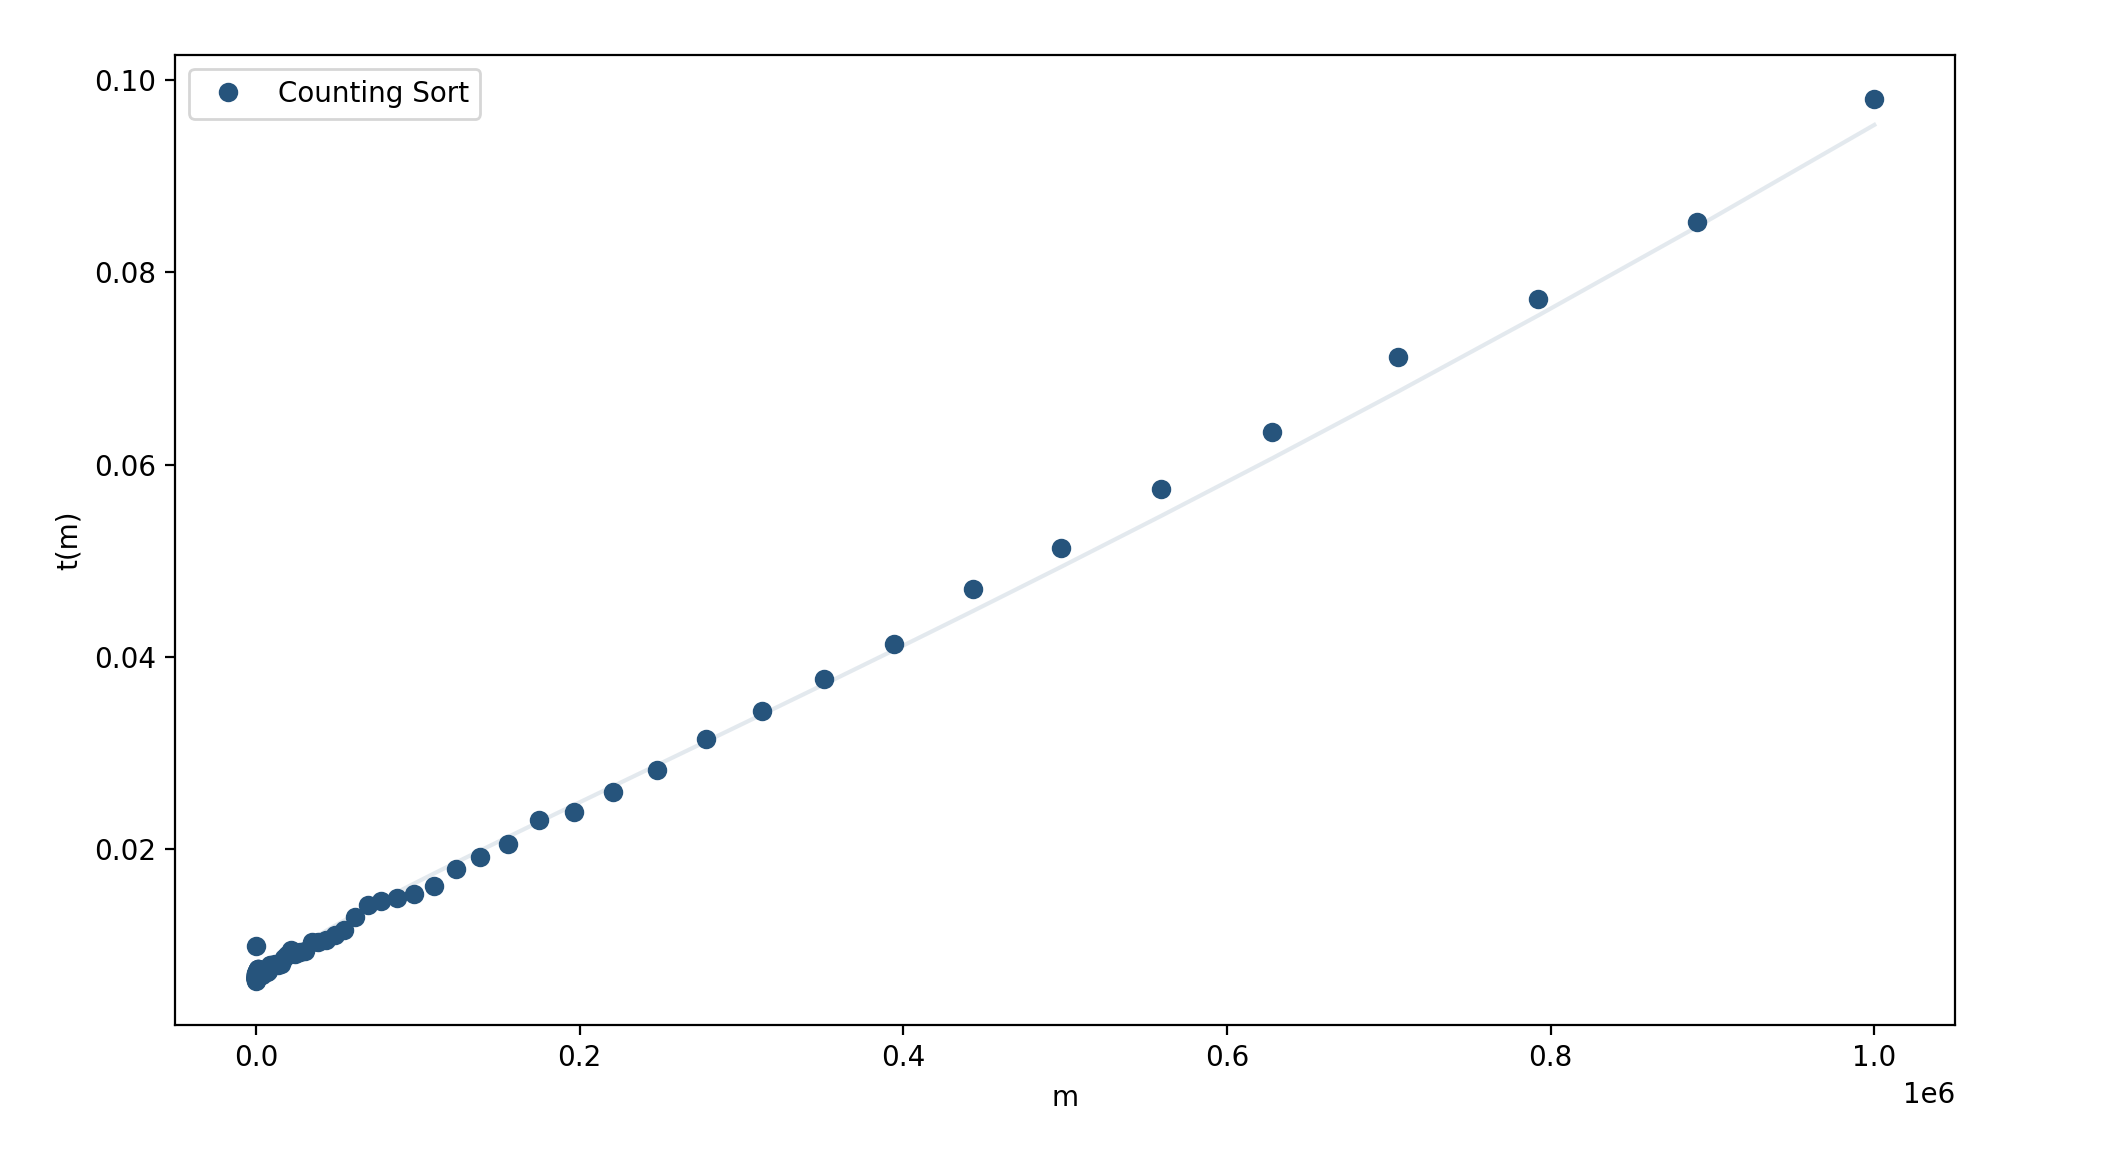
\includegraphics[width=0.8\textwidth]{images/grafico_counting_sort_m.png}
    \caption{Performance del Counting Sort al variare di \(m\).}
    \label{fig:counting_sort_m}
\end{figure}

% chapter Counting Sort (end)

\chapter{Quick Sort}\label{chap:Quick Sort} % (fold)

Il Quick Sort è un algoritmo di ordinamento basato sulla strategia del divide et impera (ovvero: dividere il problema in sottoproblemi più piccoli, risolverli ricorsivamente e combinare i risultati).
A partire da un array \(A\), si seleziona un pivot, in questo caso l'elemento finale del sottoarray \(A[p...q]\), e si procede alla partizione: tutti gli elementi minori o uguali al pivot vengono spostati a sinistra, quelli maggiori a destra. L'indice finale del pivot è restituito dalla funzione partition, e l'algoritmo viene poi richiamato ricorsivamente sulle due sottosequenze risultanti.

L'implementazione utilizzata è in-place (cioè non richiede spazio aggiuntivo proporzionale all'input), ma non stabile (l'ordine relativo tra elementi uguali può cambiare).

La funzione \texttt{uniformedQuickSort} è una versione ausiliaria pensata per rendere uniforme l'interfaccia tra gli algoritmi testati: riceve come parametro anche \(k\) (massimo valore degli elementi), che tuttavia non viene utilizzato in questo caso, in quanto Quick Sort non dipende dal dominio dei valori.

\section{Analisi della complessità}

Sia \(n\) la dimensione dell'array da ordinare:

\begin{itemize}
    \item Caso medio: \(O(n \cdot log(n))\), si verifica quando il pivot divide l'array in modo bilanciato.
    \item Caso migliore: \(O(n \cdot log(n))\), con partizioni esattamente simmetriche.
    \item Caso peggiore: \(O(n^2)\), quando il pivot è sempre il minimo o il massimo elemento (partizione altamente sbilanciata).
    \item Spazio ausiliario: \(O(log(n))\) nel caso medio per la profondità dello stack ricorsivo; \(O(n)\) nel caso peggiore.
\end{itemize}

\noindent A differenza di altri algoritmi come Counting Sort o Radix Sort, Quick Sort non richiede conoscenza del range dei valori interi e lavora unicamente tramite confronti tra elementi.

\section{Analisi sperimentale}

Per analizzare empiricamente il comportamento del Quick Sort sono stati eseguiti due esperimenti distinti:

\begin{itemize}
    \item Esperimento 1: variazione della dimensione dell'array \(n\), mantenendo fisso \(m = 100000\).
    \item Esperimento 2: \(n = 10000\) costante, con variazione di \(m\).
\end{itemize}

\noindent In entrambi i casi, i parametri sono distribuiti secondo una progressione geometrica.
Per ogni coppia \((n, m)\) sono stati generati almeno 100 campioni casuali, ciascuno eseguito più volte per stimare in modo accurato il tempo medio di esecuzione, con un errore relativo massimo \(\leq 0.001\).
Le misurazioni sono state effettuate mediante un clock monotono ad alta precisione (\texttt{time.perf\_counter()} in Python).

Poiché Quick Sort opera esclusivamente tramite confronti, il valore massimo m non influisce direttamente sulla complessità. Tuttavia, può avere effetti indiretti sulla distribuzione dei dati (ad esempio, la presenza di molti duplicati o valori ripetuti), il che può influenzare l'efficienza della partizione. \\

\noindent I risultati ottenuti mostrano che:

\begin{itemize}
    \item Nel primo grafico, i tempi di esecuzione crescono come \(O(n log n)\), in linea con il comportamento teorico nel caso medio.
    \item Nel secondo grafico, la variazione di \(m\) non produce cambiamenti significativi nei tempi di esecuzione, a conferma del fatto che l'algoritmo non dipende dal dominio numerico.
\end{itemize}

\section{Grafico dei tempi di esecuzione}

È stato generato un grafico in cui varia la lunghezza dell'array da ordinare, indicata con \(n\), mentre il parametro \(m\) (range dei valori) è mantenuto costante. L'ordinamento è stato eseguito utilizzando l'algoritmo Quick Sort su array contenenti numeri casuali. Sull'asse delle ascisse è riportato il valore di \(n\), da 100 a 1.000.000, mentre sull'asse delle ordinate è rappresentato il tempo medio di esecuzione, espresso in secondi.

\begin{figure}[H]
    \centering
    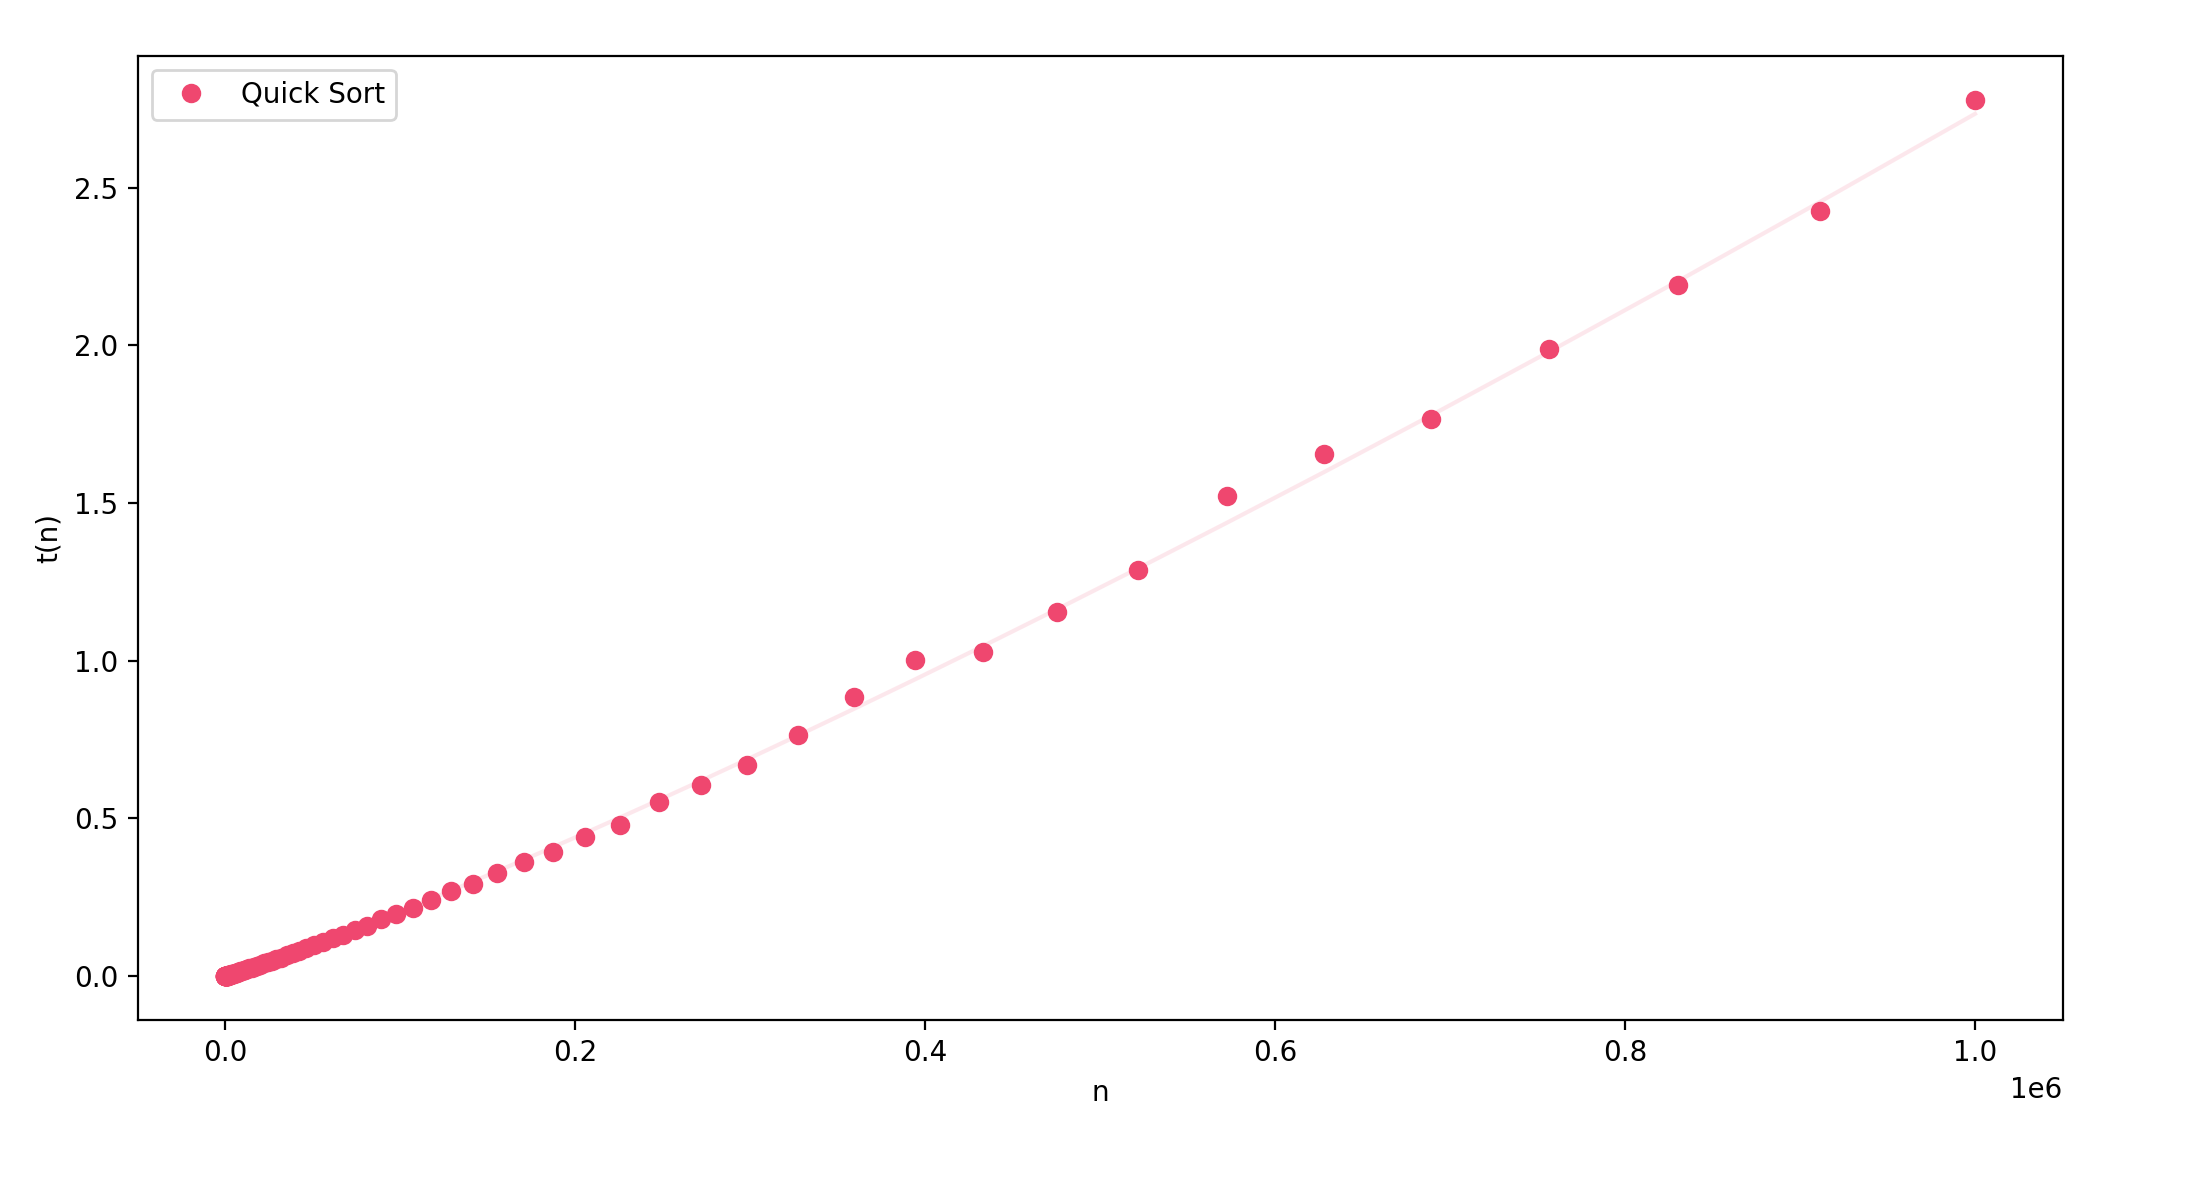
\includegraphics[width=0.8\textwidth]{images/grafico_quick_sort_n.png}
    \caption{Performance del Quick Sort al variare di \(n\).}
    \label{fig:quick_sort_n}
\end{figure}

\noindent Successivamente, è stato realizzato un grafico in cui varia il range dei valori interi presenti nell'array, indicato con \(m\), mantenendo costante la dimensione dell'array a \(n=10000\). Nel grafico riportato di seguito, sull'asse delle ascisse è rappresentata la variazione di \(m\), da 10 a 1.000.000, in scala scientifica. Sull'asse delle ordinate è riportato il tempo medio di esecuzione dell'ordinamento, espresso in secondi.

\begin{figure}[H]
    \centering
    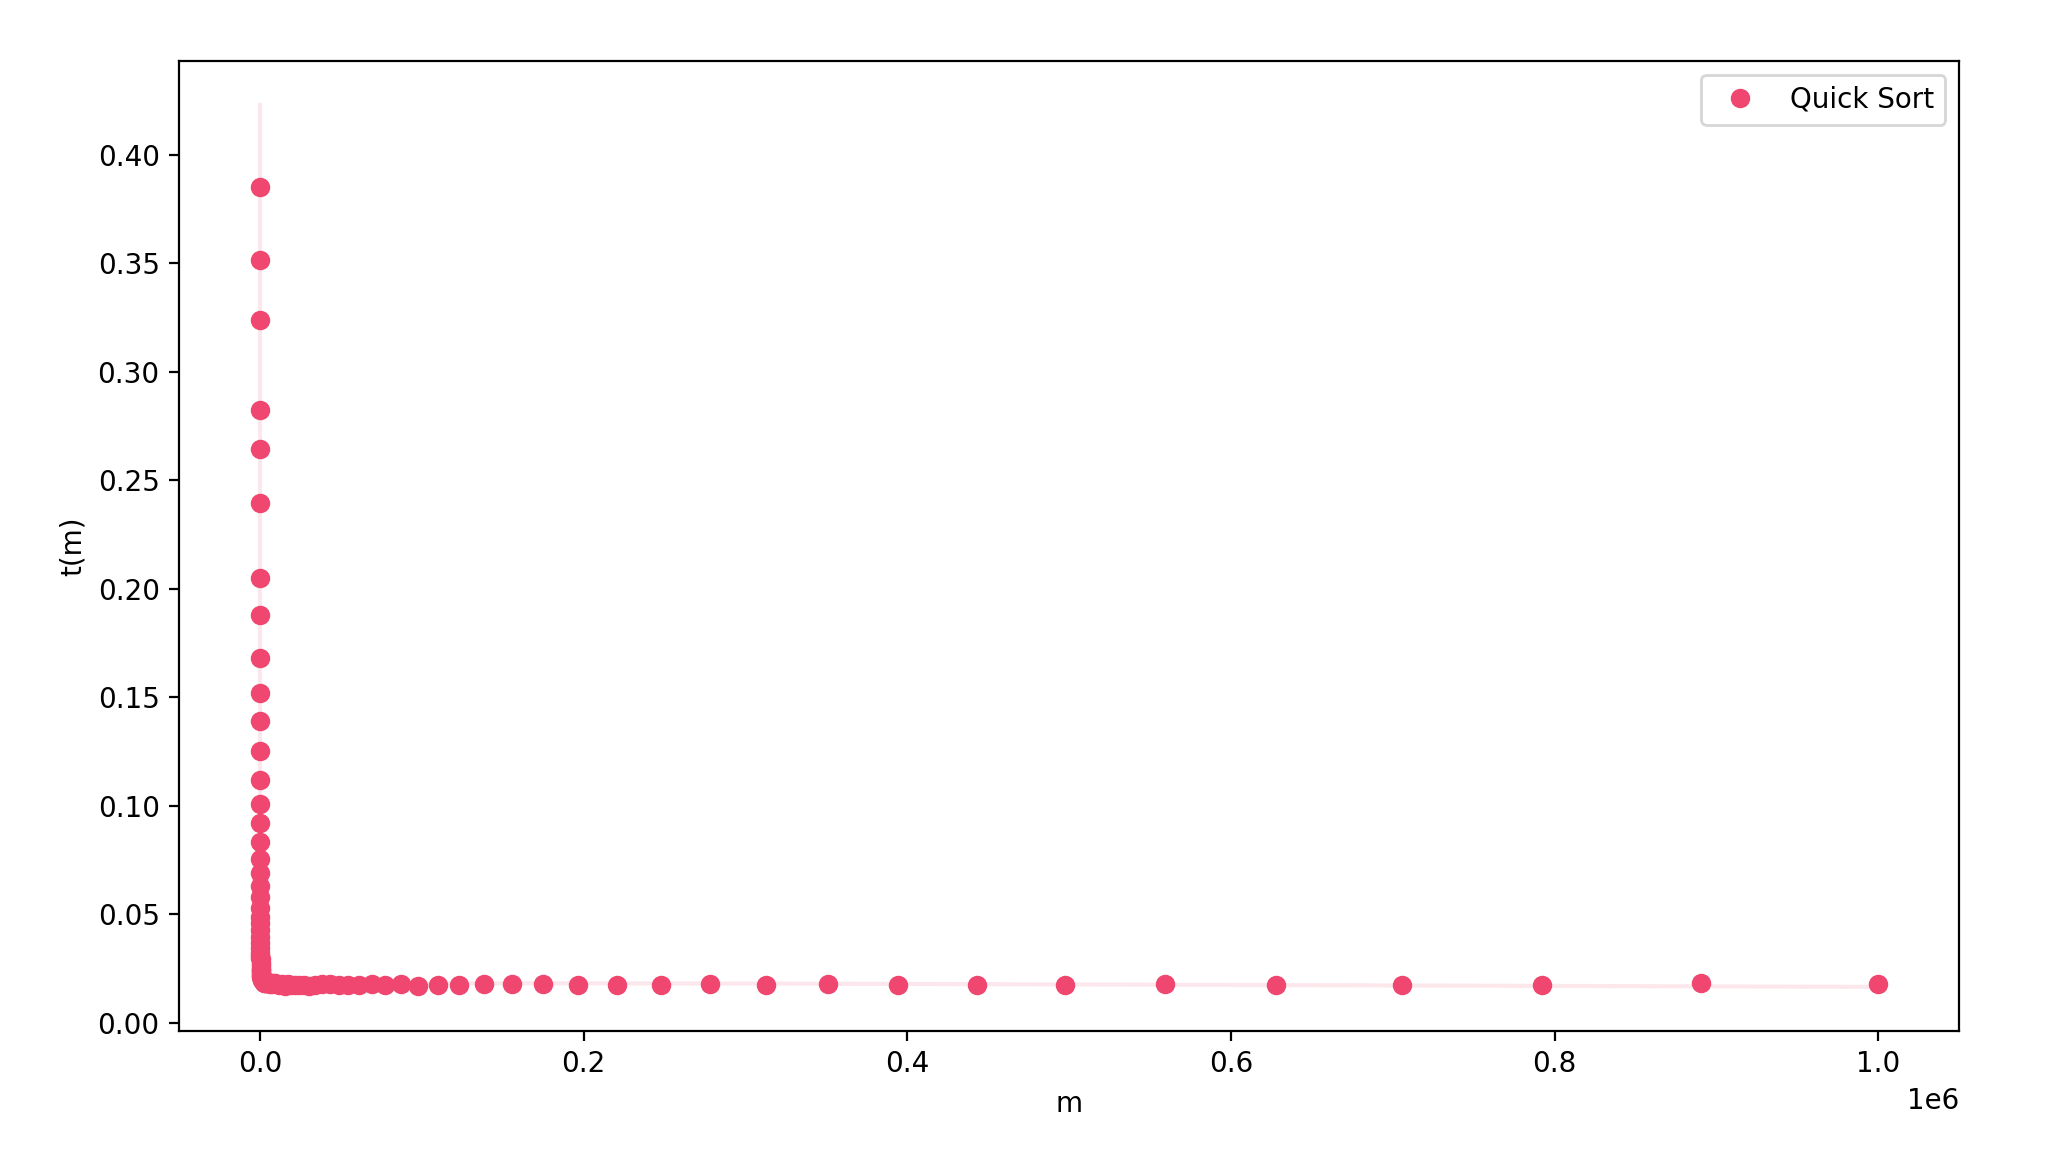
\includegraphics[width=0.8\textwidth]{images/grafico_quick_sort_m.png}
    \caption{Performance del Quick Sort al variare di \(m\).}
    \label{fig:quick_sort_m}
\end{figure}

\noindent Si osserva un'anomalia nel grafico quando il numero di valori distinti presenti nell'array (\(m\)) è molto basso. Sarà opportuno approfondire l'origine di questo comportamento, che potrebbe essere legato alla scarsa diversità dei dati e al conseguente degrado delle prestazioni dell'algoritmo.

% chapter Quick Sort (end)

\chapter{Quick Sort 3 Way}\label{chap:Quick Sort 3 Way} % (fold)

TODO

% chapter Quick Sort 3 Way (end)

\chapter{Radix Sort}\label{chap:Radix Sort} % (fold)

TODO

% chapter Radix Sort (end)

\chapter{Conclusioni}\label{chap:Conclusioni} % (fold)

TODO

% chapter Conclusioni (end)

\end{document}
